\chapter{Literature Review}

\section{Introduction}
Over the past decade, machine learning and deep learning have shown great potential in addressing challenges in early disease detection and pest identification in agriculture. This literature review critically examines current wheat disease classification and pest detection research using deep learning techniques. It explores the evolution from traditional methods to modern AI-driven approaches, highlighting the strengths and limitations of each. Key challenges such as limited data availability, model complexity, and interpretability are discussed in the context of real-world applications. The review also identifies major trends and research gaps in the field. By synthesizing these findings, it aims to provide insights into the future of smart agriculture. This chapter lays the groundwork for the thesis’s proposed deep learning-based system. The goal is to enhance disease and pest management in wheat crops. Ultimately, it aims to contribute to more efficient, sustainable farming practices.

\section{Approaches in Data Collection and Preprocessing }
This section discusses various methods employed in the literature for gathering data, handling challenges such as low-quality or irrelevant images, and preprocessing techniques that prepare datasets for effective utilization in classification and detection tasks.
\subsection{Data Collection}
The first step in developing deep learning models for wheat disease classification and pest detection involves gathering high-quality data from various sources. \textbf{For wheat disease classification}, data can include images captured via drones or mobile cameras, as well as public datasets such as Kaggle's "Wheat Leaf Dataset" used by \parencite{ ramadan2024improving} and "Wheat Disease Detection" employed by \parencite{reis2024integrated}. Manual image acquisition is also common; for example, \parencite{hassan2024wheat} combined field-captured images, Kaggle datasets, and internet-sourced images, while \parencite{onler2024wheat} captured natural field images using an iPhone8.

\textbf{For pest detection}, advanced imaging techniques like hyperspectral imaging captured via UAVs have proven effective, as demonstrated by \parencite{zhang2019deep}. Public datasets such as IP102, which contains over 75,000 pest images, have been widely used, as highlighted by \parencite{ali2023faster}. Additionally, \parencite{albattah2023custom} combined drone-captured images with the IP102 dataset to provide in-field pest images under various conditions. Other methods include task-specific devices with high-definition cameras and multispectral light traps, as employed by \parencite{liu2019pestnet}, or locally collected pest images from crops and online sources such as Google Images and Flickr.

\subsection{Data Preprocessing}
Once the data is collected, it undergoes preprocessing to ensure it is ready for model training. This includes image normalization, resizing, noise reduction, and correcting lighting or angle variations. For wheat disease detection, preprocessing often involves removing low-quality images where disease features are unclear \parencite{yao2024yolo} and clipping unnecessary portions of images to focus on relevant regions. Techniques like histogram equalization \parencite{yao2024yolo} and CLAHE \parencite{reis2024integrated} enhance contrast and brightness, improving disease feature visibility.

To mitigate the effects of lighting variations, \textbf{contrast enhancement techniques} are applied to improve image uniformity \parencite{fang2023lightweight}. Histogram equalization and adaptive histogram equalization (CLAHE) are used to enhance image contrast and highlight disease-specific features \parencite{nigam2023deep}. Images are typically resized to standard dimensions such as 640x640 pixels \parencite{hassan2024wheat} or 224x224 pixels \parencite{reis2024integrated}, ensuring compatibility with deep learning models. Common dimensions for CNN-based models include 224×224 pixels, while high-resolution detection models often use 640×640 pixels \parencite{goyal2021leaf}.


\textbf{Data augmentation} is widely applied to address class imbalances and increase dataset diversity using methods such as random rotation, cropping, flipping, and contrast adjustments \parencite{ramadan2024improving} \parencite{hassan2024wheat}. In particular, rotating images by 90° and 270° has been found to significantly enhance model performance \parencite{nigam2023deep}. Augmentation techniques also include zooming, brightness adjustments, and contrast modification to improve model robustness \parencite{nigam2023deep}.

\textbf{Noise reduction} is also crucial; for example, background noise is minimized using segmentation masks or bounding boxes \parencite{hassan2024wheat}. Additionally, background noise is reduced through contrast adjustment and segmentation methods \parencite{fang2023lightweight}. Annotation of datasets is performed using tools like LabelImg and Labelme to ensure precise labeling of wheat disease regions \parencite{yao2024yolo} \parencite{hassan2024wheat}. Proper annotation ensures accurate labeling of diseased and healthy regions, which improves classification accuracy \parencite{goyal2021leaf}.

For pest detection, preprocessing shares similar steps but also incorporates specific adjustments. Images are resized to dimensions like 224x224 pixels \parencite{turkoglu2019plant} \parencite{albattah2023custom} or 320x320 pixels \parencite{ali2023faster} to match model input requirements. \textbf{Advanced augmentation techniques}, including horizontal flipping \parencite{liu2019pestnet} and affine transformations \parencite{ali2023faster}, are used to increase dataset size and diversity. \parencite{albattah2023custom} performed manual object-level labeling using the LabelImg tool to define regions of interest for pest identification. Background noise is reduced through manual adjustments and segmentation, ensuring a focus on pests in the images. These preprocessing steps ensure that the datasets for pests are diverse and of high quality, enabling deep learning models to perform effectively in real-world scenarios.

Segmentation, labeling, and splitting the data into training, validation, and test sets are the final steps common to both wheat disease and pest detection, ensuring robust and reliable model training.

\section{Approaches in Wheat Disease Classification}

Various classification models have been employed in the literature to address wheat disease classification effectively. These approaches, preprocessing techniques, datasets, classification categories, and results, are summarized in Table~\ref{tab:Table 01}, which provides a comparative overview of the most recent and relevant studies in this domain.

\textbf{Transfer Learning Approaches:} \parencite{ramadan2024improving} adopted a transfer learning strategy, utilizing pre-trained CNN models such as DenseNet121, ResNet50V2, MobileNetV2, and Xception. These models were fine-tuned for wheat leaf disease classification using both augmented and non-augmented datasets, demonstrating significant adaptability and enhanced performance (see Table~\ref{tab:Table 01}). Additionally, \parencite{nigam2023deep} proposed a transfer learning approach using EfficientNet variants for classifying wheat rust diseases. They introduced the WheatRust21 dataset with 6,556 field images across four classes: healthy, stripe, leaf, and stem rust. EfficientNet B4 achieved the highest testing accuracy of 99.35\% on the augmented dataset. The model outperformed classical CNNs and demonstrated strong generalization. However, the dataset is not publicly available, limiting external validation (see Table~\ref{tab:Table 01}).


\textbf{Hybrid Models:} \parencite{reis2024integrated} introduced a hybrid model that combined pre-trained deep learning models, including DenseNet201, InceptionV3, RegNetY080, and Xception, for feature extraction. For classification, traditional machine learning algorithms such as SVM, Random Forest, and Decision Tree were applied. Ensemble learning methods were also employed to improve model performance (see Table~\ref{tab:Table 01}). Similarly, \parencite{goyal2021leaf} proposed a hybrid CNN model that integrates feature extraction techniques with machine learning classifiers, enhancing classification performance for wheat disease images (see Table~\ref{tab:Table 01}).

\textbf{Custom Deep Convolutional Networks:} \parencite{zhang2019deep} developed a custom deep convolutional neural network (DCNN) specifically designed for yellow rust detection in wheat fields. The model integrated Inception-ResNet layers for feature extraction, effectively leveraging both Inception and ResNet architectures to process spatial and spectral data from high-resolution hyperspectral images (see Table~\ref{tab:Table 01}).


\textbf{Task-Specific CNN Architectures:} \parencite{goyal2021leaf} proposed an improved deep convolutional architecture tailored specifically for wheat disease classification. Unlike models based on transfer learning or pre-existing architectures like VGG16 or ResNet50, this model was designed entirely from scratch, addressing the unique requirements of the wheat disease classification task (see Table~\ref{tab:Table 01}).


\textbf{Few-Shot Learning:} \parencite{alharbi2023wheat} used a few-shot learning approach with EfficientNet as the backbone. The model utilized a Siamese network architecture, sharing a feature extractor for both the support and query sets, which enabled efficient learning with minimal labeled data. Additionally, an attention mechanism was integrated to enhance feature selection and reduce computational costs (see Table~\ref{tab:Table 01}).

\textbf{Lightweight CNNs for Efficient Classification:} \parencite{fang2023lightweight} introduced a lightweight multiscale CNN model optimized for mobile and edge computing applications. By integrating Inception modules with residual blocks and attention mechanisms like CBAM and ECA, the model enhanced feature extraction while reducing computational costs, achieving 98.78\% accuracy on wheat disease classification tasks​. Likewise,\parencite{jouini2023wheat} proposed a deep learning approach using MobileNetV2 and EfficientNet variants to build a lightweight yet accurate CNN-based model for wheat leaf disease detection in smart agriculture, achieving 94\% test accuracy and supporting real-time use in IoT environments (see Table~\ref{tab:Table 01}).

\begin{table}[htbp]
    \caption{Related Work to Wheat Disease Classification}
    \centering
    \resizebox{1.05\textwidth}{!}{%
    \begin{tabular}{|p{2.5cm}|p{4.2cm}|p{3.8cm}|p{1.5cm}|p{3.2cm}|p{3cm}|p{3.6cm}|}
    \hline
    \textbf{References} & \textbf{Approach} & \textbf{Image Preprocessing} & \textbf{Size (images)} & \textbf{Categories} & \textbf{Dataset} & \textbf{Results} \\
    \hline
    \parencite{ramadan2024improving} & Pre-trained CNNs (DenseNet121, ResNet50V2, etc.) & CycleGAN, ADASYN, SMOTE, SMOTETomek & 407 & 3 classes (healthy, stripe rust, septoria) & Wheat Leaf Dataset & 100\% accuracy (MobileNetV2 + CycleGAN) \\
    \hline
    \parencite{reis2024integrated} & DL + ML ensemble hybrid model & CLAHE, hypercolumn & 2400 & 3 classes (healthy, yellow rust, brown rust) & Wheat Disease Dataset & Accuracy: 99.72\% \\
    \hline
    \parencite{zhang2019deep} & Inception-ResNet CNN with spatial-spectral learning & 3D HSI blocks (64×64×125) & / & 2 classes (healthy, rust) & / & Accuracy: 85\% \\
    \hline
    \parencite{goyal2021leaf} & Improved CNN for wheat classification & / & 12,000 & 10 classes (e.g., tan spot, leaf rust, etc.) & LWDCD2020 & Accuracy: 97.88\% \\
    \hline
    \parencite{alharbi2023wheat} & Few-shot learning with EfficientNet & Attention mechanism & 1530 & 18 classes & PV, CGIAR, manual, Google Images & Accuracy: 93.19\% \\
    \hline
    \parencite{jouini2023wheat}  & CropNet (EfficientNetB0 + CNN) & Resize (256x256), StandardScaler & / & 5 classes (Healthy, Septoria, etc.) & / & Accuracy: 99.80\% \\
    \hline
    \parencite{fang2023lightweight} & IRCE: Inception-ResNet with CBAM/ECA & Contrast, flip, rotate, enhance & >12,000 & 7 classes (e.g., tan spot, smut, etc.) & LWDCD2020, PV, CGIAR & Accuracy: 98.76\% \\
    \hline
    \parencite{nigam2023deep} & EfficientNet deep transfer learning & Resize, contrast, rotate, brightness & 6556 & 4 classes (e.g., rusts, healthy) & WheatRust21 & Accuracy: 99.35\% \\
    \hline
    \end{tabular}%
    }
    \label{tab:Table 01}
\end{table} 
    
The studies are complementary as they address different challenges in wheat disease classification. Figure ~\ref{fig:Figure01} summarizes the main approaches used in this field, providing a taxonomy that includes transfer learning, hybrid models, custom CNN architectures, few-shot learning, lightweight CNNs, and attention mechanisms. Transfer learning helps overcome limited data by leveraging pre-trained models, while hybrid models combine deep learning and traditional machine learning to enhance performance. Custom and task-specific CNNs are tailored to the unique features of wheat diseases, improving accuracy. Few-shot learning enables effective classification with minimal labeled data, and lightweight CNNs optimize real-time detection for mobile and edge devices, balancing performance with computational efficiency. Each approach targets a specific problem, enhancing the overall classification process.    

\begin{figure}[H]
    \centering
    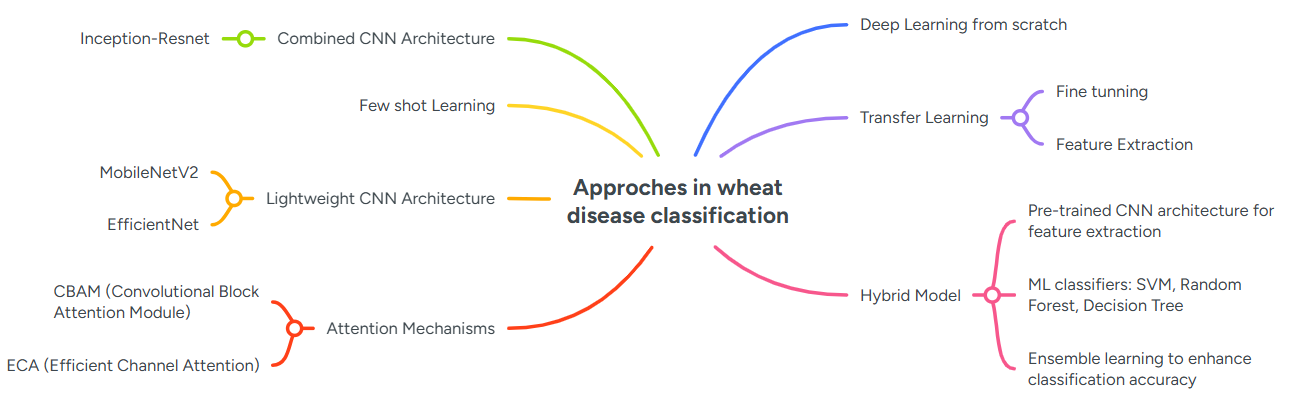
\includegraphics[width=1.0\textwidth]{chapters/chapter3/images/Figure01.png}
    \caption{Taxonomy of Approaches for Classifying Wheat Diseases. \protect\parencite{haider2021wheat}}
    \label{fig:Figure01}
\end{figure}



\section{Approaches in Wheat Disease Detection}

Wheat disease detection focuses on identifying and localizing infected areas using object detection models. Recent studies have explored YOLO-based architectures due to their high speed and accuracy, particularly in real-time field applications.

\textbf{YOLO-Based Models:} \parencite{yao2024yolo} proposed an enhanced YOLO-based model, YOLO-Wheat, incorporating the C2f-DCN module for improved feature extraction. The SCNet attention mechanism was used to focus on relevant features, while a small target detection layer improved the model's detection accuracy for minor diseases (see Table~\ref{tab:Table 02}).

\textbf{Advanced YOLO Architectures:} \parencite{onler2024wheat} utilized YOLOv8m for wheat leaf detection. The model integrated advanced modules such as CSPDarknet53 for feature extraction, PANet for multi-scale feature fusion, and Spatial Pyramid Pooling–Fast (SPPF) for enhanced model performance and efficiency (see Table~\ref{tab:Table 02}).

\textbf{Hybrid MobileNet-YOLO Models:} \parencite{hong2022lightweight} proposed a hybrid MobileNetv3-YOLOv4 model that combined depth-wise separable convolutions and the focal loss function to improve disease detection accuracy while maintaining a lightweight design (see Table~\ref{tab:Table 02}).

These methods highlight the effectiveness of object detection models in accurately identifying disease-affected regions, supporting timely and targeted agricultural interventions.

\begin{table}[htbp]
    \caption{Related Work to Wheat Disease Detection}
    \centering
    \resizebox{1.05\textwidth}{!}{%
    \begin{tabular}{|p{2.5cm}|p{4.5cm}|p{4.2cm}|p{1.7cm}|p{3.2cm}|p{3cm}|p{2.8cm}|}
    \hline
    \textbf{References} & \textbf{Approach} & \textbf{Image Preprocessing} & \textbf{Size (images)} & \textbf{Categories} & \textbf{Dataset} & \textbf{Results} \\
    \hline
    \parencite{yao2024yolo} & YOLO-Wheat: C2f-DCN for feature extraction, SCNet for attention, small target detection layer & Filtering low-quality images, histogram equalization, annotation using LabelImg & 3622 & 5 Classes (yellow rust, brown rust, smut, stem rust, healthy) & Custom dataset & mAP of 93.28\% \\
    \hline
    \parencite{hassan2024wheat} & YOLOv8 for localization, deep learning for segmentation/classification & Downscaling, normalization, Otsu, cropping, VARI, data augmentation, manual annotation (Labelme) & 584 & 3 Classes (Healthy, Resistant, Susceptible leaves) & Manual images, wheat dataset, online images & mAP of 95.5\% \\
    \hline
    \parencite{onler2024wheat} & YOLOv8 & Cropping, flipping, contrast adjustments, resizing to 640x640 & 224 & 1 Class (Powdery Mildew) & Custom dataset & mAP of 76.5\% \\
    \hline
    \parencite{hong2022lightweight} & MobileNetv3-YOLOv4, uses MobileNetv3 and focal loss for lightweight model & Cropping, affine transform, flipping, noise, blur, contrast/brightness adjustment & 866 & 1 Class (Fusarium head blight) & Custom dataset & mAP of 93.69\% \\
    \hline
    \end{tabular}%
    }
    \label{tab:Table 02}
\end{table}



\section{Approaches in Wheat Insect Pest Detection}

Detection models for pest identification have been developed using various approaches, combining deep learning architectures with innovative enhancements (see Table~\ref{tab:Table 03}).

\textbf{Region Proposal-Based Approaches:} Models like PestNet \parencite{liu2019pestnet} and Faster-PestNet \parencite{ali2023faster} utilized region proposal methods for pest detection and classification. PestNet incorporated a Channel-Spatial Attention (CSA) module to improve feature extraction, a Region Proposal Network (RPN) for pest region identification, and a Position-Sensitive Score Map (PSSM) for bounding box regression and classification. Contextual regions of interest (RoIs) were also integrated to enhance predictions. PestNet achieved a mean Average Precision (mAP) of 75.46\% on the MPD2018 dataset with 16 pest classes. Faster-PestNet enhanced the Faster R-CNN framework by using MobileNet as a lightweight backbone, reducing computational complexity while maintaining detection accuracy. It achieved a higher mAP of 82.43\% on the large-scale IP102 dataset containing 102 pest categories.

\textbf{Feature Extraction and Transfer Learning:} \parencite{turkoglu2019plant} used pre-trained CNN architectures such as AlexNet, VGG16, and ResNet50 for deep feature extraction. These models were fine-tuned by replacing the final layers with task-specific fully connected, softmax, and output layers. Transfer learning enabled efficient adaptation for pest detection tasks. Traditional machine learning models such as Support Vector Machine (SVM), Extreme Learning Machine (ELM), and K-Nearest Neighbor (KNN) were applied for classification using the extracted features. Their approach achieved a high mean Average Precision (mAP) of 97.86\% on a real-world dataset that covering 8 pest categories.

\textbf{Keypoint-Based Detection:} \parencite{albattah2023custom} proposed a keypoint-based detection approach using a custom CornerNet model with DenseNet-100 as the backbone, which detects pests by estimating paired keypoints (top-left and bottom-right corners) instead of relying on traditional anchor-based bounding boxes. Unlike conventional detectors such as YOLO and Faster R-CNN, which use multi-stage pipelines, first generating region proposals, then classifying and refining them, CornerNet performs detection in a single stage. This streamlined process improves computational efficiency and is particularly suited for detecting small or overlapping pests. However, despite its architectural advantages, the method achieved a mean Average Precision (mAP) of 57.8\% on the IP102 dataset, which is lower than other recent models, indicating that further optimization may be needed for practical deployment.

\begin{table}[htbp]
    \centering
    \caption{Related Work for Pest Detection}
    \resizebox{1.05\textwidth}{!}{%
    \begin{tabular}{|p{3cm}|p{4.5cm}|p{4cm}|p{1.5cm}|p{2cm}|p{3cm}|p{1.5cm}|}
    \hline
    \textbf{References} & \textbf{Approach} & \textbf{Image Preprocessing} & \textbf{Size (images)} & \textbf{Categories} & \textbf{Dataset} & \textbf{Results (mAP)} \\
    \hline
    \parencite{liu2019pestnet} & PestNet uses a Channel-Spatial Attention module, Region Proposal Network, Position-Sensitive Score Map, and Contextual RoIs for improved pest detection. & Data is augmented using the "mirror" strategy, generating horizontally flipped images & 88670 & 16 classes & Multi-class Pest Dataset 2018 (MPD2018) & 75.46\% \\
    \hline
    \parencite{turkoglu2019plant} & Deep features were extracted using nine pre-trained CNN architectures (e.g., AlexNet, VGG16, ResNet50), followed by transfer learning with task-specific fine-tuning, and classification was performed using SVM, ELM, and KNN. & Images were resized to meet deep network input requirements (e.g., 224x224 or 227x227 pixels) using bilinear interpolation. & 1956 & 8 classes & Real-world dataset of plant diseases and pests from Turkey. & 97.86\% \\
    \hline
    \parencite{ali2023faster} & Faster-PestNet is a Faster R-CNN model with MobileNet & Human specialists manually labeled the dataset, resized images to 224x224 pixels, and used 320x320 dimensions for model training. & 75000 & 102 classes & IP102 \newline Link & 82.43\% \\
    \hline
    \parencite{albattah2023custom} & A custom CornerNet model with DenseNet-100 as the backbone & Images were resized to 224×224 pixels, and the LabelImg tool was used for annotating regions of interest (RoIs). & 75222 & 102 classes & IP102 \newline Link & 57.8\% \\
    \hline
    \end{tabular}%
    }
    \label{tab:Table 03}
\end{table}
    

\section{Core Limitations and Research Gaps in Wheat Disease and Pest Detection}
Deep learning has shown great promise in automating wheat disease and pest detection, offering timely and precise solutions for sustainable agriculture. However, key challenges still limit its widespread adoption.

\noindent Based on the previously discussed studies, various approaches have been explored for wheat disease classification, ranging from transfer learning using pre-trained convolutional neural networks (CNNs) to the development of custom architectures tailored specifically for disease classification tasks. The proposed models for wheat disease classification that detect five or fewer disease classes generally achieve accuracies of 99\% or higher. However, models aiming to detect more than five classes tend to achieve lower accuracies, typically below 98\%, highlighting the challenge of achieving high accuracy when dealing with more complex classification tasks.

\noindent Additionally, the number of disease classes addressed in most proposed models for wheat detection remains limited compared to wheat disease classification, with a maximum of five classes, primarily due to the difficulty of manual annotation and the high computational resources required to train models on larger, more diverse datasets. Although several public datasets for wheat disease classification are available, such as those on Kaggle, we reviewed and consulted these sources and found that many contain low-quality images, inconsistent labeling, or irrelevant data, which can hinder model training and performance. This necessitates manual cleaning and preprocessing of the datasets before they can be effectively utilized, increasing the time and effort needed for research.

\noindent  Moreover, the performance of these models is often affected by inconsistencies in image data. Therefore, diversifying image data is crucial, photos should be taken under varying lighting conditions, such as on sunny and cloudy days, and from different distances, including both close-up and wider shots. For these reasons, creating a custom dataset by selecting diverse images from different public datasets is important to ensure this variability and improve model robustness.

\noindent Similarly, deep learning approaches for pest management have made notable strides, especially with the introduction of region proposal networks (RPNs) and keypoint-based detection techniques. Models like PestNet and Faster-PestNet have demonstrated the ability to accurately detect and classify pests by incorporating feature extraction techniques such as the Channel-Spatial Attention (CSA) module. However, pest detection in wheat remains underexplored, with few studies focusing on wheat-specific pests. Existing research tends to focus on all types of insect pests rather than targeting pests specific to wheat. Additionally, there are no publicly available pre-annotated datasets for wheat pest detection, and all existing approaches rely on manual annotations, which can be time-consuming and prone to inconsistencies.

Another key challenge is the trade-off between accuracy and computational efficiency. While models like Faster-RCNN and Mask-RCNN achieve high accuracy (up to 99.68\%), they demand significant computing power, which limits their use in resource-constrained agricultural settings. Many are also not optimized for real-time deployment \parencite{li2022recommending}.

\section{Conclusion}
In conclusion, integrating image-based detection systems powered by advanced deep learning models presents a promising solution for combating wheat diseases and insect pests. The reviewed methodologies highlight the importance of data acquisition, preprocessing techniques, and model selection for accurate and efficient detection. While significant progress has been made, challenges such as dataset limitations, computational cost, and model generalization remain. Future research should improve model robustness, data augmentation strategies, and real-time deployment to facilitate practical applications in agricultural fields. As technology continues to evolve, these detection systems are expected to play an increasingly vital role in sustainable agriculture.